\section{Introduction}
Many of our daily activities involve changing our posture to a target pose without losing balance. For example, to stand up from a chair, we carefully maintain balance while switching from a sitting pose to a standing pose. There are a large variety of motions of similar kind, such as lean-to-stand, kneel-to-stand and stand-to-handstand. These motions involve complex motor skills, balance strategy and rich interactions with the environments. Understanding and synthesizing these motions can have far-reaching impacts in robotics, especially in rehabilitation, exoskeleton and humanoid robots.

We present a system that can automatically design controllers for humanoid robots to achieve these locomotion tasks. In this paper, a controller is a desired joint trajectory that a robot follows from the initial to the target pose. A successful controller, in addition, needs to keep the robot balanced during the motion. Finding a successful controller is challenging due to the high dimensional control problem, nonlinear dynamics, discontinuous contact forces and delicate balance control. It often requires tedious manual tuning and a large number of expensive robot experiments. 

To tackle these challenges, we develop a simulation-driven approach that consists of three main components, physical simulation, controller optimization and simulation calibration. We first build a \emph{physical simulation} to simulate the dynamics of the robot and its interaction with the environments. We use \emph{controller optimization} to search for the optimal joint trajectories to fulfil the task in the simulation. However, even though this optimal controller works effectively in the simulation, it can perform poorly on a robot in the real environment. This ``Reality Gap'' \cite{Jakobi95} is caused by various simplifications in simulation algorithms, such as simplified actuator models, inaccurate physical parameters, and ignored hardware limitations, noise and latency. 

We use \emph{simulation calibration} to cross the Reality Gap. Simulation calibration is a dynamic system identification method. During calibration, we collect the real performance data on the robot, and use it to improve our physical simulator. We optimize a set of simulation parameters to minimize the discrepancy between the simulation results and the collected real data. Through calibration, the simulator can capture the real world dynamics more faithfully. This calibrated simulator is used again in controller optimization to improve the quality of the controller. Unlike traditional system identification, which is a separate step from controller design, our simulation calibration is tightly coupled with the controller optimization. We directly peform the optimal controller that is found in the simulation to collect real data for system identification. In this way, the simulation is calibrated at the vicinity of the current optimal controller. The computation is focused at the important regions of the control space and thus fewer robot experiments are needed. We evaluate our system using four locomotion tasks: lean-to-stand, sit-to-stand, kneel-to-stand and stand-to-handstand. Although these tasks are distinctively different, our system can find successful controllers for all the tasks efficiently and automatically. 

\begin{figure*}[!t]
  \centering
  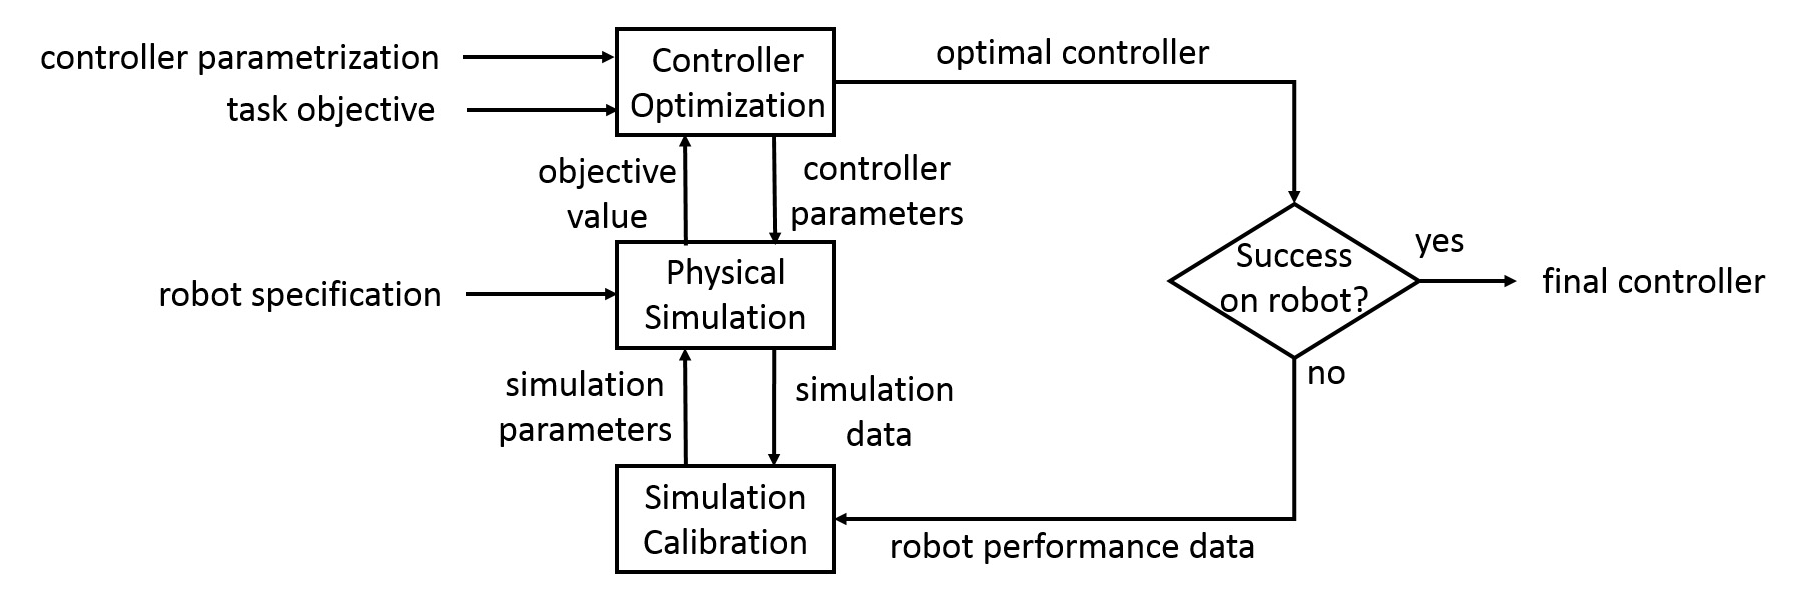
\includegraphics[width=0.7\textwidth]{figures/controllerTransfer}
  \caption{Overview of our algorithm.}
  \label{fig:controllerTransferOverview}
\end{figure*}

The main contribution of this paper is a complete pipeline that can automatically design robot controllers for a wide range of locomotion tasks. Starting from task specifications, our system can find controllers that operate on the robot, with minimal human intervention. It replaces the tedious manual tuning with automatic optimization processes, and drastically reduces the number of expensive robot experiments. This simulation-driven approach can effectively cut the time and the cost of designing robot controllers.
